\documentclass[a4paper]{article}
\usepackage{graphicx}
\usepackage[hidelinks]{hyperref}
\usepackage{xcolor}
\usepackage{url}
\usepackage{outlines}
\usepackage{listings}
\usepackage{fontspec}
\usepackage{parskip}
\usepackage[dvipsnames]{xcolor}
\usepackage{minted}
\lstset{basicstyle=\ttfamily,
	showstringspaces=false,
	commentstyle=\color{blue},
	keywordstyle=\color{RubineRed}
}
\lstset{emph={
	agree,tos,nginx,d,non,interactive,m,rsa,keyout,out,subj,days,newkey,nodes,openssl,req,x509,ARG,COPY,EXPOSE,RUN,FROM,CMD,nc,tcp,udp,http,docker},emphstyle=\color{purple}
}
\lstdefinestyle{yaml}{
     basicstyle=\color{RubineRed}\ttfamily,
     rulecolor=\color{blue},
     string=[s]{'}{'},
     stringstyle=\color{black},
     comment=[l]{\#},
     commentstyle=\color{blue},
     morecomment=[l]{-}
 }
\newcommand{\abc}{\hfill \break}
\newcommand{\cute}{\cite}
\usepackage{fancyhdr}
\usepackage{geometry}
\geometry{
	a4paper,
	total={170mm,257mm},
	left=20mm,
	top=20mm,
	bottom=39mm,
}

\setlength{\headheight}{82.70538pt}

\fancypagestyle{oida}{
	\fancyhf{}
	\fancyhead[L]{\fontsize{7.5}{7.5}htl donaustadt\\ Donaustadtstraße 45\\
		1220 Wien\\~\\ Abteilung: Informationstechnologie\\ 
	Schwerpunkt: Netzwerktechnik}
	\fancyhead[R]{
\includegraphics[scale=0.45]{images/logo.png}}

	\fancyfoot[L]{\today}
	\fancyfoot[C]{\jobname}
	\fancyfoot[R]{Page: \thepage}
}

\begin{document}
\bibliographystyle{IEEEtran}
\pagestyle{oida}
\section*{Exercise 6: GNU/Linux - Securing active components}
\par\noindent\rule{\textwidth}{0.4pt}

Laboratory protocol
\begin{figure}[h]
	
\includegraphics[scale=0.28]{images/mika.png}
	\centering
	\caption{Grouplogo}
\end{figure}

\vspace*{\fill}
Subject:	ITSI

Class:	3AHITN

Name:	Stefan Fürst, Marcel Raichle

Gruppenname/Nummer: Team 7/7

Supervisor: 	SPAC, ZIVK

Exercise dates:	6.12.2024. 13.12.2024, 20.12.2024, 3.1.2025, 4.1.2025, 5.1.2025

Submission date: 4.1.2025


\newpage
\tableofcontents

\newpage

\section{Task definition}
\paragraph*{Task 0 - Preparation}\abc
Ensure your server from Exercises 4 and 5 is configured with SSH. Verify that you can connect to the server via SSH using a client with a GUI.

\paragraph*{Task 1 – Installing a Web Server}\abc
Install a web server (e.g., Apache or Nginx) and deploy a static HTML page displaying your group number, team members, and an AI-generated image. (Bonus: Deploy a dynamic PHP page.) Demonstrate access to the page from a client browser.

\paragraph*{Task 2 – Securing with Basic Authentication}\abc
Set up Basic Authentication on the server. Create user accounts in the format \texttt{nnv-webuser} and for your instructors (e.g., \texttt{zivk-webuser}). Demonstrate authentication functionality. (Bonus: Capture the password using Wireshark.)

\paragraph*{Task 3 – Encrypting with HTTPS}\abc
Enable HTTPS with a self-signed certificate, including your group number. Demonstrate encrypted access and explain potential issues. Install the certificate on a client to show why this action is not required in the public internet.

\paragraph*{Bonus Task – Local DNS Setup (Optional)}\abc
Set up DNS on the server using \texttt{bind9} for local access via \texttt{xxx.itsi3.local}. Demonstrate DNS resolution and access the website by domain name.\footnote{This task definition was summarized by ChatGPT using the prompt: "Summarize this task definition in English and LaTeX and make it short and abstract."}
\section{Summary}
As preparation for the exercise, I optimized the Docker workflow by using Docker Compose for easier management, improved the readability of the Dockerfile, and, most importantly, created a \texttt{.env} file along with a build script that utilizes it, so I no longer hardcode my passwords in the Dockerfile. Additionally, I disabled password authentication and now copy the \texttt{authorized\_keys} file into the container, allowing for key-based authentication from the start and enabling me to disable password authentication.\abc
We need to install a web server, for which I chose \texttt{nginx}. I used it in conjunction with \texttt{php-fpm} to deploy a dynamic PHP webpage. The webpage includes our group number, names, and an AI-generated image. However, since this information should only be accessible with credentials, I implemented Basic Authentication to secure it. For this, the \texttt{apache2-utils} package was used to generate a \texttt{.htpasswd} file containing the credentials.\abc
We demonstrated with Wireshark that the credentials were transmitted in plain text while using HTTP. To address this, a self-signed SSL certificate was generated using \texttt{openssl}, with the group number included in the \texttt{OU} field of the certificate. The server was then configured to use HTTPS. We showed that the credentials could no longer be read with Wireshark, as the traffic was now encrypted.\abc
Lastly, we set up a domain, created a DNS record to point to the server, and generated a proper SSL certificate with Let's Encrypt, ensuring it is trusted and does not display a warning in the browser.

\newpage

\section{Complete network topology of the exercise}

\begin{figure}[h]
	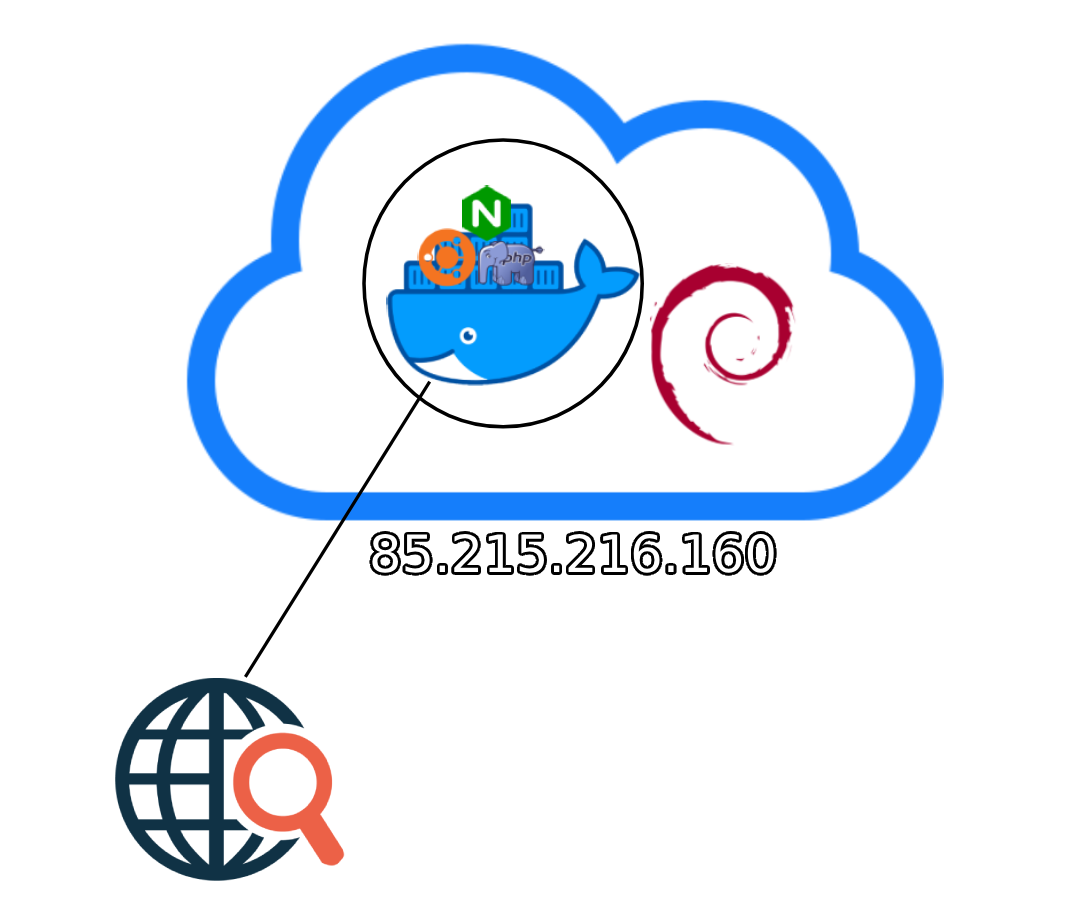
\includegraphics[scale=0.3]{images/topology.png}
	\centering
	\caption{Network topology of this exercise}
\end{figure}

\newpage

\section{Exercise Execution}

\subsection{Preparation}
The requirements for this exercise are a headless Linux server with hardened SSH, which only allows connections via key pairs. However, I removed the OTP authentication added in the last exercise, as it was overkill for this use case and became a burden to use.
\begin{figure}[h]
	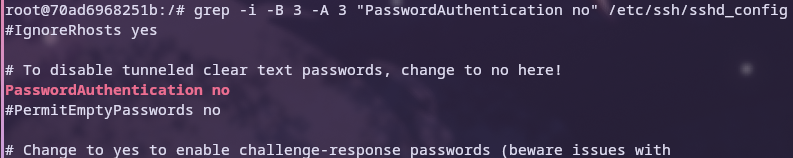
\includegraphics[scale=0.26]{images/sshnopw.png}
	\centering
	\caption{Password authentication disabled}
\end{figure} 
\subsection {Testing the SSH connectivity.}
\begin{figure}[h]
	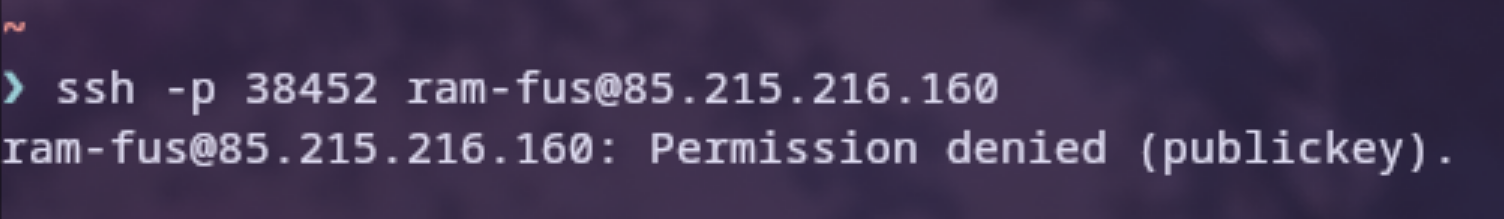
\includegraphics[scale=0.13]{images/nokey.png}
	\centering
	\caption{No SSH key available}
\end{figure}
\begin{figure}[!hbp]
	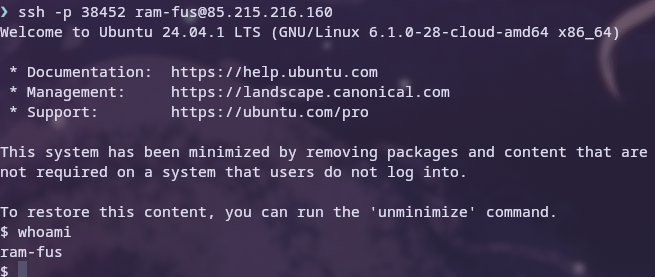
\includegraphics[scale=0.3]{images/yeskey.png}
	\centering
	\caption{ram-fus authenticating via SSH key}
\end{figure}

\begin{figure}[!htbp]
	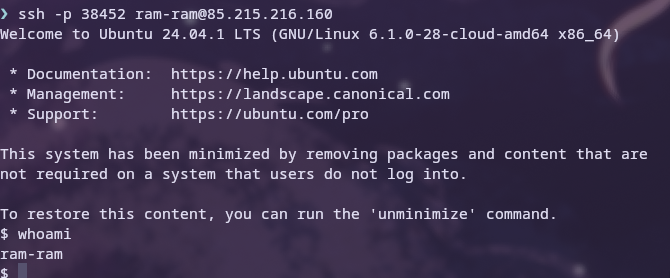
\includegraphics[scale=0.3]{images/yeskey2.png}
	\centering
	\caption{ram-ram authenticating via SSH key}
\end{figure}\newpage
\subsubsection{Changes to the Docker setup}
To improve the quality of life when working on this project, I switched from aliasing a long and hard-to-read run command to using Docker Compose, which allows you to define and run multi-container applications. Since it's in a YAML file, it is more readable and easier to work with, even in this use case where I only have one container.\cite{Docker-Compose}
\begin{lstlisting}[language=bash]
services:
    #setting the name image and restart policy
    webserver:
        container_name: itsi
        image: itsi:latest
        restart: no
    #setting exposed ports
    ports:
        - "38452:38452"
        - "80:80"
        - "443:443"
\end{lstlisting}
Furthermore, instead of having all of the credentials in the Dockerfile, I created a \texttt{.env} file in which the passwords are set. To utilize that, I made a build script that passes the variables from the file to the Dockerfile \cite{docker-arg}.
\begin{lstlisting}[language=bash]
#!/bin/bash
export $(cat .env | xargs)

docker buildx build -t itsi:latest\
	--build-arg ROOT_PW=$ROOT_PW \
	--build-arg RAM_WEBUSER_PW=$RAM_WEBUSER_PW \
	--build-arg ZIVK_WEBUSER_PW=$ZIVK_WEBUSER_PW \
	--build-arg RAM_FUS_PW=$RAM_FUS_PW \
	--build-arg RAM_RAM_PW=$RAM_RAM_PW \
	--build-arg RAM_ALOIS_PW=$RAM_ALOIS_PW \
	--build-arg RAM_CHRIS_PW=$RAM_CHRIS_PW \
	--build-arg RAM_BERTA_PW=$RAM_BERTA_PW .
\end{lstlisting}
These build-time arguments are referenced in the Dockerfile like this:
\begin{lstlisting}[language=bash]
ARG ROOT_PW
ARG RAM_WEBUSER_PW
ARG ZIVK_WEBUSER_PW
ARG RAM_FUS_PW
ARG RAM_RAM_PW
ARG RAM_ALOIS_PW
ARG RAM_CHRIS_PW
ARG RAM_BERTA_PW
...
RUN echo 'root:$ROOT_PW' | chpasswd
...
\end{lstlisting}
Here is what the \texttt{.env} file looks like for this project:
\begin{lstlisting}
...
ROOT_PW='some password'
...
\end{lstlisting}
Note that the quotes are only necessary if the password contains characters like \texttt{\&}, which the shell will interpret.
With this change, I can add the \texttt{.env} file to my \texttt{.gitignore} file so I don't accidentally commit my passwords again and handle passwords in a Dockerfile properly.
\newpage
To still utilize my alias script, I changed every instance of \texttt{docker run} to \texttt{docker compose up -d}, \texttt{docker stop itsi \&\& docker rm itsi} to \texttt{docker compose down}, and added the use of the build script to it.
\begin{lstlisting}[language=bash]
#!/bin/bash
alias relaunch="sh -c 'docker stop itsi && docker rm itsi &&\
		       ./build.sh &&\
		       docker compose up -d && docker exec -it itsi /bin/bash'"
alias rebuild="sh -c './build.sh &&\
                      docker compose up -d && docker exec -it itsi /bin/bash'"
alias stop="sh -c 'docker compose down'"
\end{lstlisting}
Furthermore, instead of having to upload my container every time I rebuild, I added these three lines to copy the \texttt{authorized\_keys} file with the devices I use to the container, so that every time I relaunch, I can just immediately SSH into it.
\begin{lstlisting}[language=bash]
COPY ./mapped-files/authorized_keys /root/.ssh/authorized_keys
COPY ./mapped-files/authorized_keys /home/ram-fus/.ssh/authorized_keys
COPY ./mapped-files/authorized_keys /home/ram-ram/.ssh/authorized_keys
\end{lstlisting}
Lastly, the line in the Dockerfile that specifies the exposed ports is edited to expose ports 80 and 443, as they will be required for this exercise.
\begin{lstlisting}[language=bash]
EXPOSE 38452 80 443
\end{lstlisting}
\newpage
\subsection{Installing an active component}

Now, it's required to install a web server. I chose Nginx because I am most familiar with it, and due to its high performance and simplicity of use.\abc
It’s installed and run by adding these lines to the Dockerfile and including \texttt{service nginx start} on the last line.\footnote{While \texttt{init.d} has been deprecated in distributions such as RHEL and Oracle Linux, on Ubuntu it's not yet deprecated but considered legacy. Since this is a Docker container that's supposed to be isolated, adding \texttt{systemd} would break that isolation since it changes many low-level parameters. Almost all of its features besides process management are useless to me, so I opted for \texttt{init.d} since it doesn't require any further setup, doesn't break isolation, or add unnecessary weight.}
\begin{lstlisting}[language=bash]
...
RUN apt install -y nginx
...
CMD service ssh start && service nginx start && tail -F /dev/null
\end{lstlisting}
After modifying the Dockerfile, rebuilding, and redeploying, if we now open the web browser and go to the server's IP, we see the following.
\begin{figure}[h]
	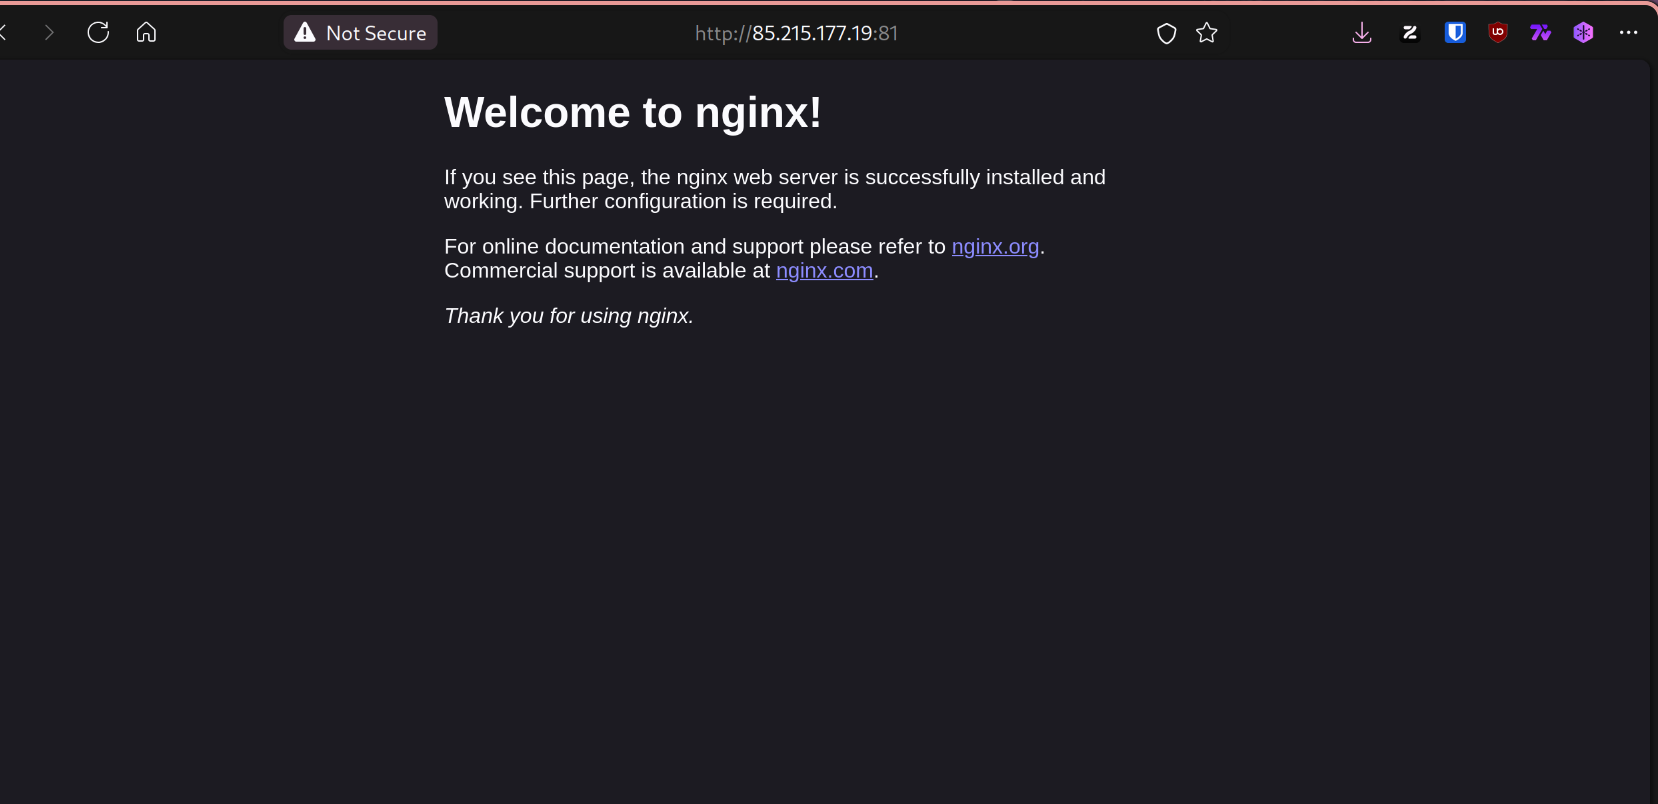
\includegraphics[scale=0.2]{images/nginx.png}
	\centering
	\caption[erm]{Default nginx site\footnotemark}
\end{figure}\abc\footnotetext{The IP and port are different since, initially, I used a VPS that already had a web server running, so I had to change the port. After that, I switched to a new VPS, which will be used for the rest of the exercise.}\abc
The HTML site displayed is located at \texttt{/var/www/html/index.nginx-debian.html}.
Additionally, I replaced the \texttt{/var/www/html} directory with \texttt{/var/www/metyr.xyz}, in which I have the following file structure:
\begin{lstlisting}[language=bash]
`-- html
   |-- private
   |   `-- private.php
    `-- public
        `-- index.php
\end{lstlisting}
These two directories are mapped onto the Docker container in the \texttt{docker-compose.yml} file, as shown below. Since they are mapped, every time the files are changed on the host, the changes carry over to the container, allowing for an easy and fast development workflow without the need to exec into the container or copy the files when creating the image.
Nginx won't serve those PHP files without further configuration, which is explained in the next section.
\begin{lstlisting}[language=bash]
volumes:
    - ./mapped-files/public:/var/www/html/public:rw
    - ./mapped-files/private:/var/www/html/private:rw
\end{lstlisting}
Additionally, I edited the Dockerfile to delete the default Nginx configuration file, located at \texttt{/etc/nginx/sites-enabled/default}, a symlink to the file \texttt{/etc/nginx/sites-available/default.conf}, and replaced it with one matching my domain name for better readability.\newpage
\begin{lstlisting}[language=bash]
RUN rm -rf /var/www/html/
RUN mkdir -p /var/www/metyr.xyz/html
RUN rm /etc/nginx/sites-available/default
RUN rm /etc/nginx/sites-enabled/default
#copying the configuration file to the container during the build process
COPY ./mapped-files/metyr.xyz /etc/nginx/sites-available/metyr.xyz
#symlinking the new configuration file to enable the site
RUN ln -s /etc/nginx/sites-available/metyr.xyz /etc/nginx/sites-enabled/metyr.xyz
\end{lstlisting}
\subsubsection{Setting up PHP-FPM with Nginx}
To give Nginx the ability to serve PHP files, the \texttt{php-fpm} (FastCGI Process Manager) package is required.
With this package installed, the following lines can be added to the server block in the Nginx configuration file.
\begin{lstlisting}[language=bash]
server{
	...
	#setting the location of the index file to serve
	index public/index.php;
	#location block, which matches requests for files ending with .php
	location ~ \.php$ {
		#include the fastcgi-php configuration file
		include snippets/fastcgi-php.conf;
		#passing the requets to the FastCGI server on set socket
		fastcgi_pass unix:/run/php/php8.3-fpm.sock;
	}
	...
}
\end{lstlisting}
Additionally, the \texttt{php-fpm} service has to be started, so the default command of the container is edited.
\begin{lstlisting}[language=bash]
CMD service ssh start && service nginx start && service php8.3-fpm start\
    && tail -F /dev/null
\end{lstlisting}
If we now rebuild the container, deploy it, and go to the IP address of the server in the browser, we can see the PHP page displayed.
The site has a public part, located at \texttt{public/index.php}, and a private part, located at \texttt{private/private.php}. The private part contains the number and members of my group, along with an AI-generated image, which is why it requires authentication to access. This will be explained in the next section.\abc
\begin{figure}[!htbp]
	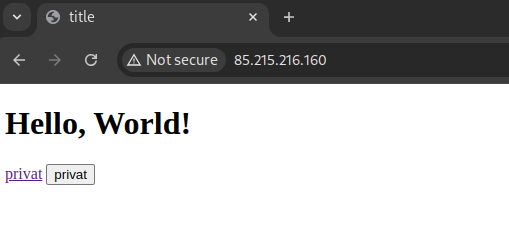
\includegraphics[scale=0.45]{images/indexphp.png}
	\centering
	\caption{Viewing the index of the website}
\end{figure}
\begin{figure}[!htbp]
	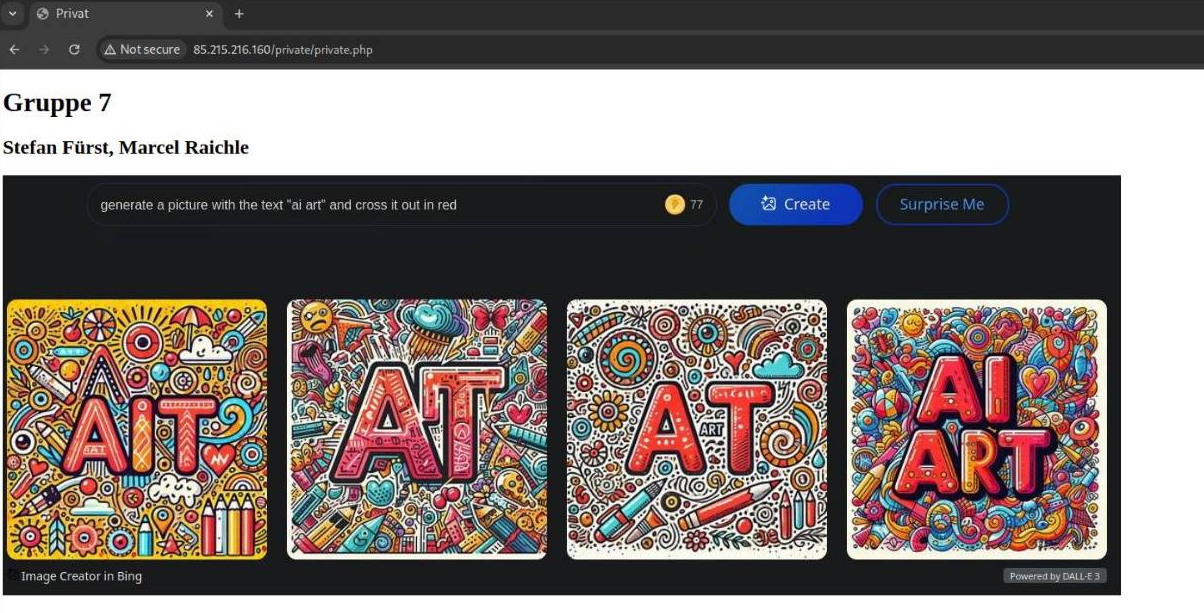
\includegraphics[scale=0.2]{images/privatphp.png}
	\centering
	\caption{Viewing the private part of the website}
\end{figure}\abc\newpage
\subsection{Securing Nginx with Basic Authentication}
To restrict access to the website or certain parts of it by implementing username/password authentication, a file containing usernames and passwords is required. This file can be generated using tools such as \texttt{apache2-utils}, which I will use for this exercise. Additionally, HTTP Basic Authentication can be combined with other access restriction methods, such as IP address or geographical location. \cite{nginx-basic-auth}
\subsubsection{Creating a Password File}
With \texttt{apache2-utils} installed, we can now generate a password file by using the \texttt{htpasswd} command with the \texttt{-c} flag to create a new file. The file path is specified as the first argument, and the username is specified as the second argument. However, to avoid having to manually type in the password, the \texttt{-i} flag is used to take the password from \texttt{stdin}, which we pass using \texttt{echo}, while using the \texttt{-n} flag to remove the trailing newline. The passwords are sourced from the \texttt{.env} file mentioned in section 4.2.1. \cite{nginx-basic-auth, htpasswd, echo-mangapge}
\begin{lstlisting}[language=bash]
RUN echo -n "$RAM_WEBUSER_PW" | htpasswd -i -c /etc/apache2/.htpasswd ram-webuser
RUN echo -n "$ZIVK_WEBUSER_PW" | htpasswd -i /etc/apache2/.htpasswd zivk-webuser
\end{lstlisting}
\subsubsection{Configuring the authentication in Nginx and testing it}
To require authentication for a specific area on the website, we need to create a location block that matches everything in the \texttt{/private} directory. To do this, Nginx URL matching is used.\cite{Nginx-url-matching}\abc
It offers the following operators:
\begin{lstlisting}[language=bash]
= #An exact match of the URI path\abc
~ #A case-sensitive regular expression match.
~* #A case-insensitive regular expression match.
^~ #Indicates that the following path should be considered the best
   #non-regular expression match.
\end{lstlisting}
\begin{lstlisting}[language=bash]
#matching everything that contains /private in the path.
location ^~ /private {
	#making php work in the location
	include snippets/fastcgi-php.conf;
	fastcgi_pass unix:/run/php/php8.3-fpm.sock;
	auth_basic "Private Area";
	#selecting the file from which to use the credentials from
	auth_basic_user_file /etc/apache2/.htpasswd;
}
\end{lstlisting}
To visualize testing the login, I added this to the private PHP page to show the currently logged-in user: \texttt{<h3>Hello <?php echo \$\_SERVER['PHP\_AUTH\_USER']; ?></h3>}.\cite{php-show-basic-auth}
\newpage
\begin{figure}[!htbp]
	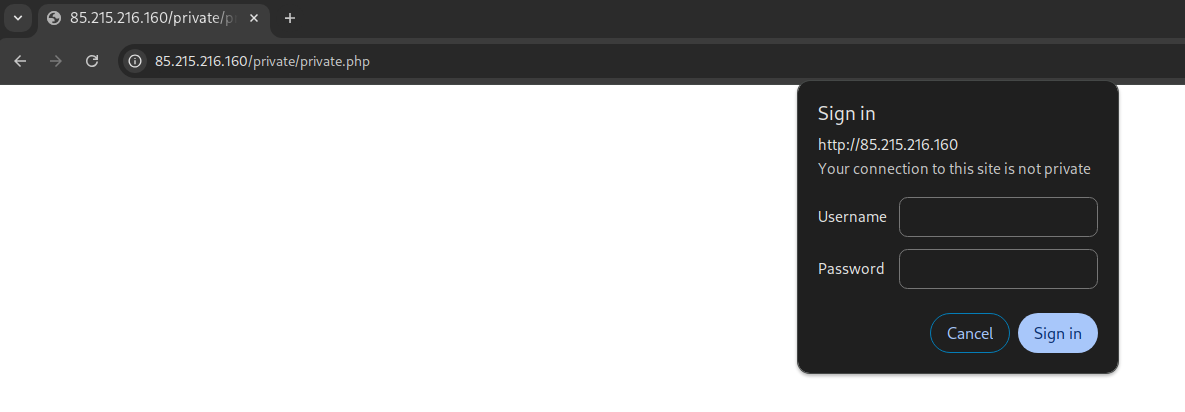
\includegraphics[scale=0.25]{images/siginprompt.png}
	\centering
	\caption{Showing the sign-in prompt}
\end{figure}
\begin{figure}[!htbp]
	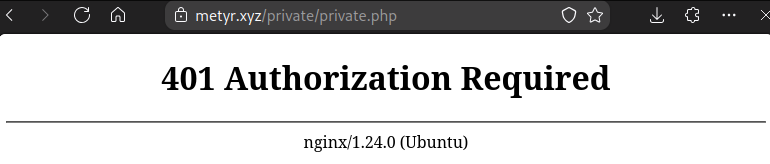
\includegraphics[scale=0.38]{images/noauth.png}
	\centering
	\caption{Failed authentication}
\end{figure}
\begin{figure}[!htbp]
	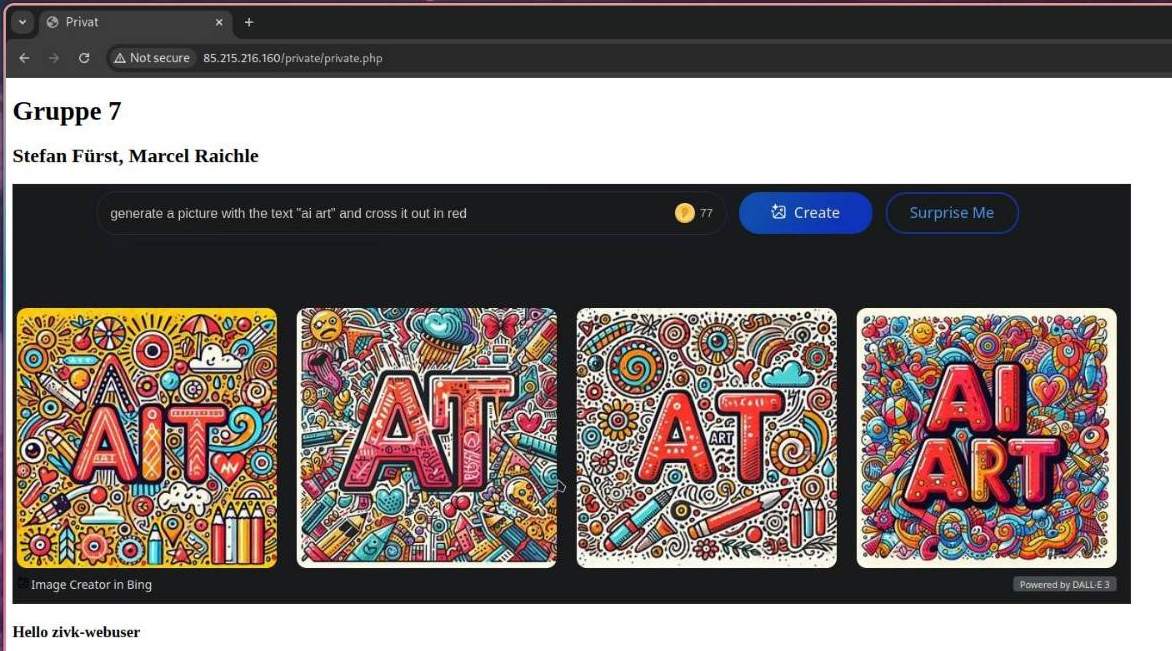
\includegraphics[scale=0.25]{images/zivk_webuser.png}
	\centering
	\caption{Logged in as zivk-webuser}
\end{figure}
\begin{figure}[!htbp]
	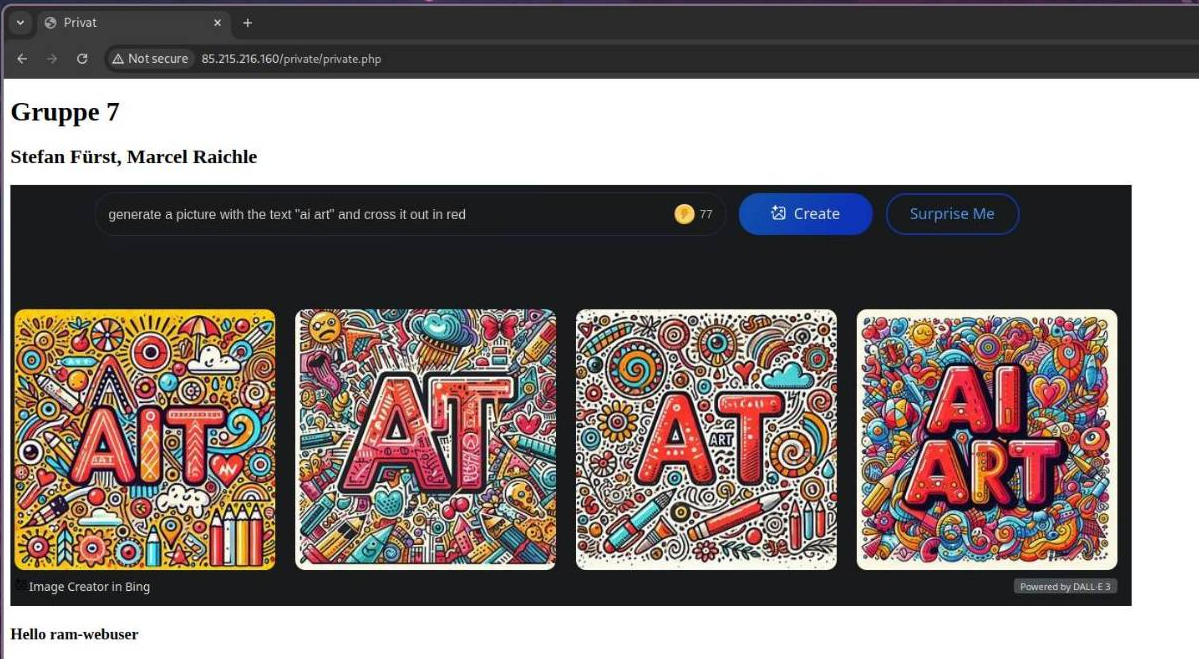
\includegraphics[scale=0.25]{images/ram_webuser.png}
	\centering
	\caption{Logged in as ram-webuser}
\end{figure}
\newpage
This is still only an HTTP site, though, which means that everything is transmitted in plain text. As a result, with a packet analyzer like Wireshark, the clear-text login credentials can be viewed. To fix this, HTTPS needs to be enabled, which will be covered in the next section.
\begin{figure}[!htbp]
	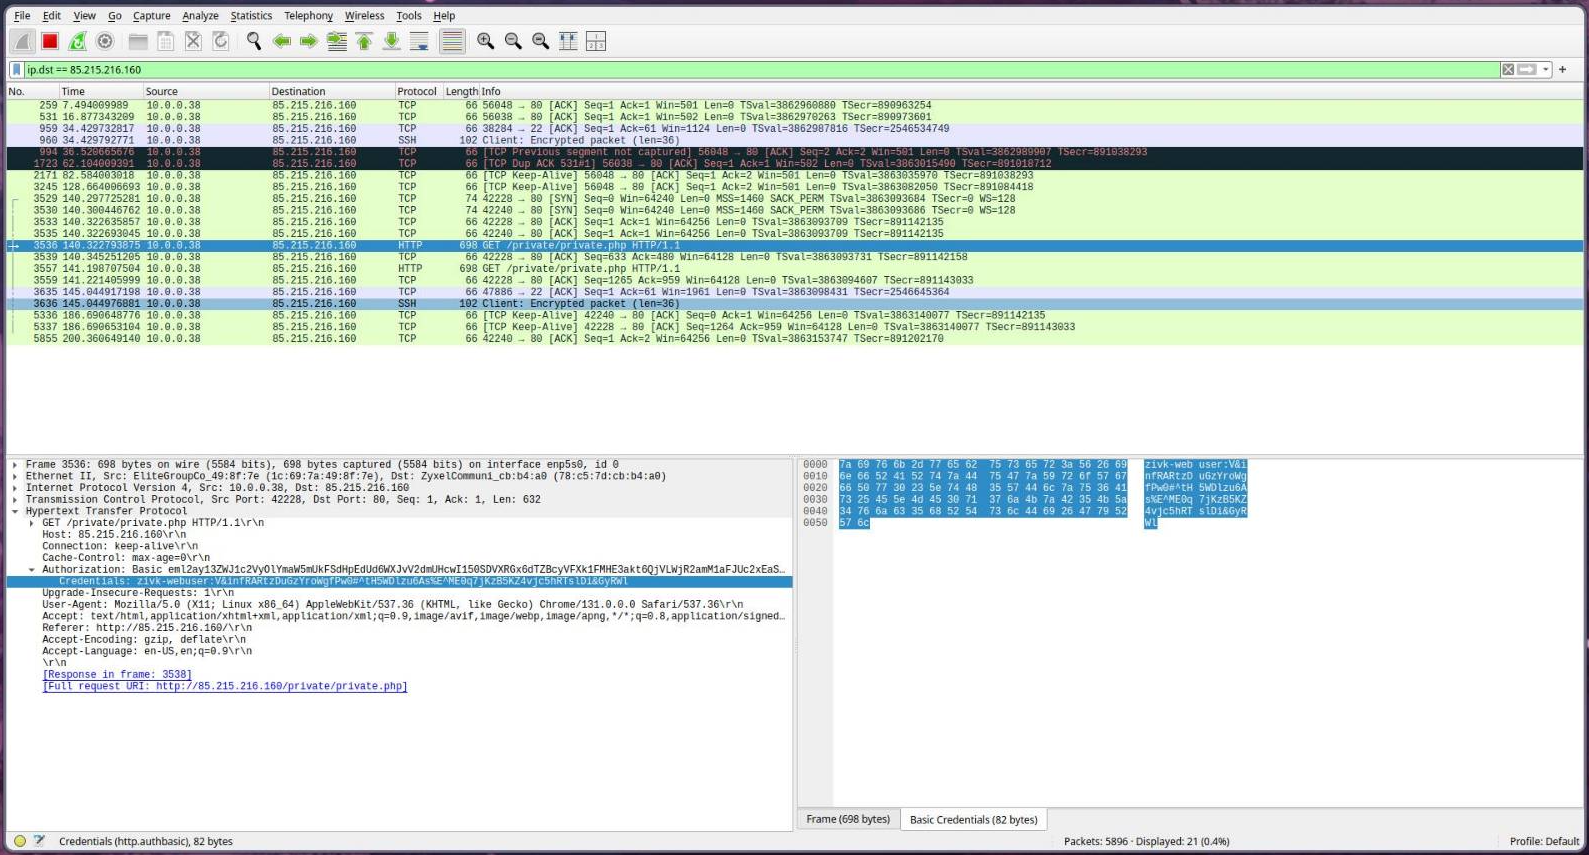
\includegraphics[scale=0.25]{images/zivk_snifa.png}
	\centering
	\caption{Reading the plaintext credentials of zivk-webuser}
\end{figure}
\begin{figure}[!htbp]
	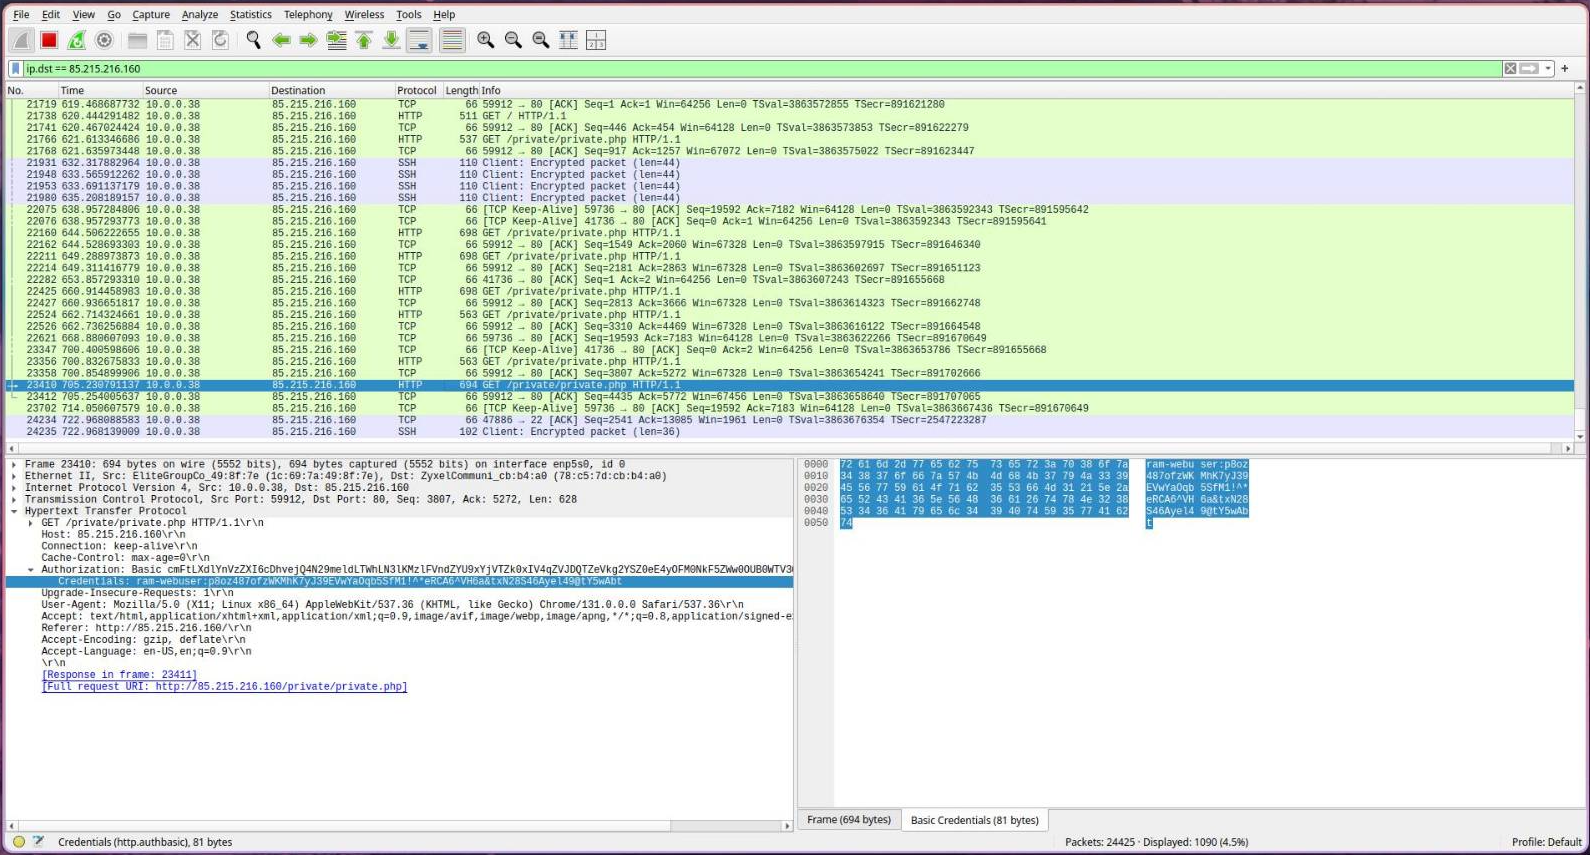
\includegraphics[scale=0.25]{images/ram_snifa.png}
	\centering
	\caption{Reading the plaintext credentials of ram-webuser}
\end{figure}
\newpage
\subsection{Configuring HTTPS with Self-Signed Certificates}
To stop an attacker from being able to read the credentials, HTTPS needs to be enabled on the server to encrypt the HTTP traffic with TLS (Transport Layer Security). Before this can be set up, an SSL certificate must first be created.
To create a self-signed SSL certificate, the cryptographic toolkit \texttt{openssl} is used with the following command:\cite{self-signed-ssl,non-interactive-ssl-gen}
\begin{lstlisting}[language=bash]
RUN openssl req -x509 -nodes -days 365 -newkey rsa:2048 \
    -keyout /etc/ssl/private/nginx-selfsigned.key \
    -out /etc/ssl/certs/nginx-selfsigned.crt \
    -subj "/C=AT/ST=Vienna/L=Vienna/O=RAM/OU=7/CN=metyr.xyz/\
          emailAddress=wedm1ebmf@mozmail.com"
\end{lstlisting}
The options used are the following:
\begin{lstlisting}[language=bash]
openssl #command-line tool to generate and manage OpenSSL certificates,
        #keys, and other files.
req #subcommand to specify useing an X.509 certificate signing request(CSR)
-x509 #telling openssl that we want to create a self-signed certificate
      #instead of generating a signing request
-nodes #tells openssl not to secure the key with a passphrase since nginx needs
       #to be able to read the file without user intervention
-days 365 #sets the length of time that the certificate will be considered valid
-newkey rsa:2048 #creates a new 2048-bit long rsa key at the same time, which 
                 #is required to sign the certificate
-keyout #output location of the private key
-out #output location of the certificate
-subj #sets certificate subject
\end{lstlisting}
The \texttt{-subj} flag is required to fill the fields of the certificate without user interaction. I put the abbreviations used in the command into square brackets and added the values I included in the command.
\begin{lstlisting}
Country Name (2 letter code) [C]: AT
State or Province Name (full name) [ST]: Vienna
Locality Name (eg, city) [L]: Vienna
Organization Name (eg, company) [O]: RAM
Organizational Unit Name (eg, section) [OU]: 7
Common Name (e.g. server FQDN or YOUR name) [CN]: 85.215.216.160
Email Address [emailAddress]:wedm1ebmf@mozmail.com
\end{lstlisting}
Now, in the Nginx configuration file, we need to make the server listen on port 443 and add the SSL certificate and key.
\begin{lstlisting}
server{
	...
	#making the server listen on port 443 for ipv4 and 6
        listen 443;
        listen [::]:443;
	#setting the ssl certificate file
        ssl_certificate /etc/ssl/certs/nginx-selfsigned.crt;
	# setting the ssl certificate key file
        ssl_certificate_key /etc/ssl/private/nginx-selfsigned.key;
	...
}
\end{lstlisting}\newpage
After setting up \texttt{https}, it's recommended to set up a 301 HTTP redirect to direct HTTP traffic to the \texttt{https} site. This is done by adding a second server block at the end of the nginx config file. However, I didn't do it since I will use \texttt{Certbot} in the end, which will set this up for me anyway.

\begin{lstlisting}
server {
	listen 80;
	listen [::]:80;
	server_name _;
	return 301 https://$server_name$request_uri;	
}
\end{lstlisting}
If we reload the Nginx configuration, our browser is going to give us a security warning since it recognizes that the certificate was not signed by a trusted organization but by ourselves. \begin{figure}[!htbp]
	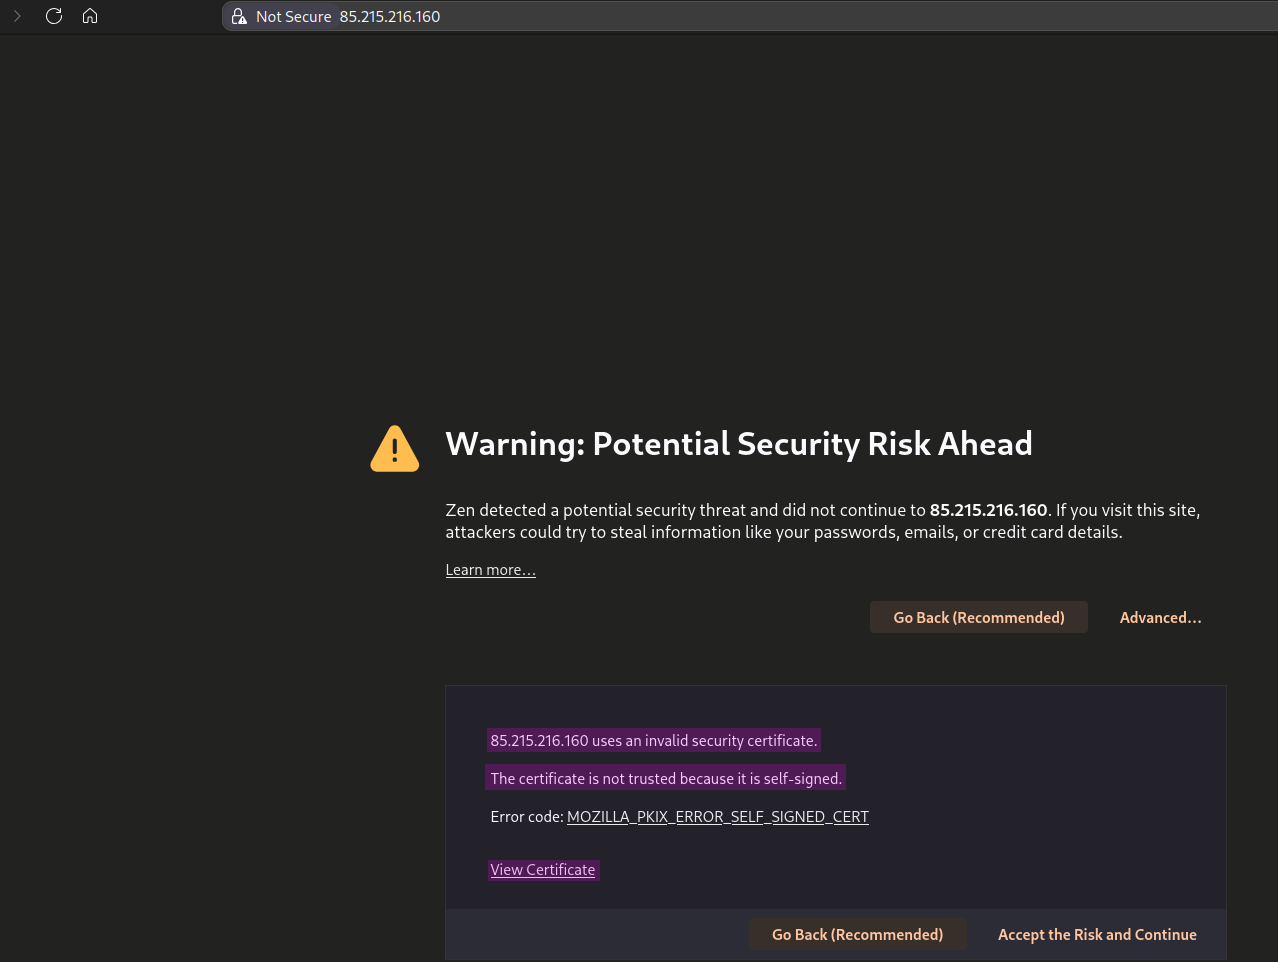
\includegraphics[scale=0.25]{images/unseccert.png}
	\centering
	\caption{Browser warning for untrusted certificate}
\end{figure}\abc
If we accept the risk and continue, we can inspect the certificate by clicking "View Certificate."
\begin{figure}[!htbp]
	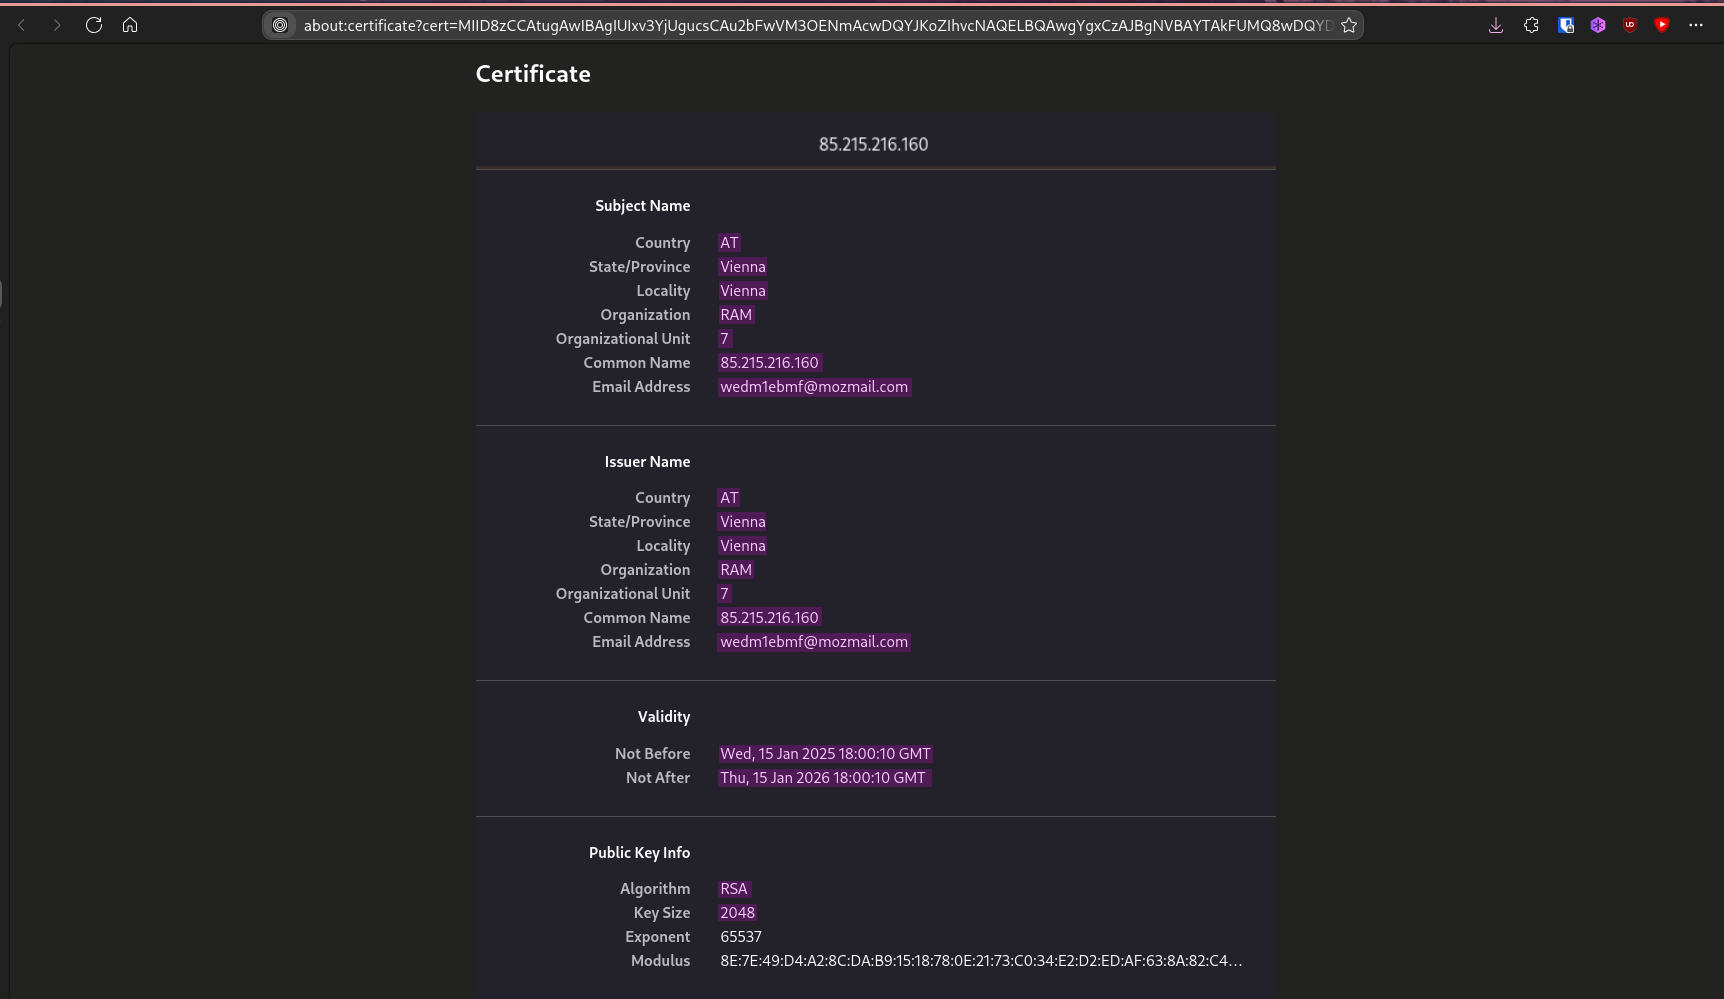
\includegraphics[scale=0.2]{images/selfcert.png}
	\centering
	\caption{Viewing the self-signed certificate}
\end{figure}
\newpage
If we open up Wireshark and inspect our traffic, we can see that we can't view any HTTP traffic. Instead, we only see TLS packets, which contain the encrypted HTTP data, and therefore the credentials can't be viewed anymore.
\begin{figure}[!htbp]
	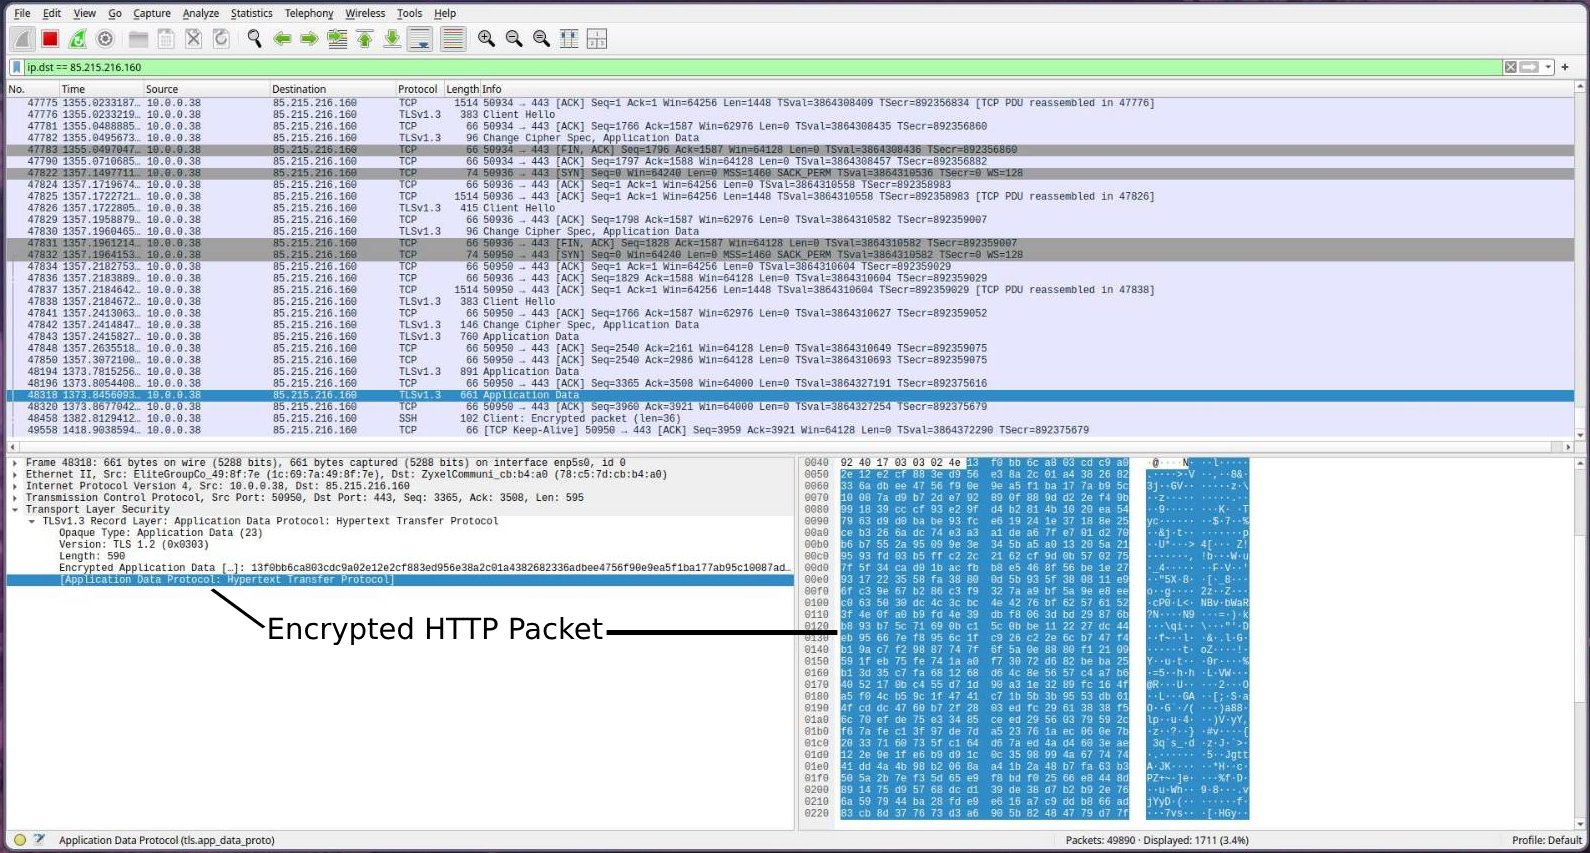
\includegraphics[scale=0.2]{images/nohaxxor.png}
	\centering
	\caption{Not being able to see the credentials anymore}
\end{figure}
\subsection{Adding a Domain}
Since I am doing this on a public VPS, I can't use a local DNS and need to use a real domain instead. I bought \texttt{metyr.xyz} from \url{https://www.namecheap.com/}.
To make Nginx use the domain name, you have to set the \texttt{server\_name} in the configuration from \texttt{server\_name \_;} to \texttt{server\_name metyr.xyz www.metyr.xyz;}.\abc
Now we need to create a DNS record for our domain.\abc
This record needs to be of the \texttt{A} type, which returns a 32-bit IPv4 address and is commonly used to map hostnames to an IP address. \cite{dns-record-types}\abc
The \texttt{@} in the Host field is used to denote the current origin, which represents the current domain. In this case, it would be \texttt{metyr.xyz}. \cite{rfc}
\begin{figure}[!htbp]
	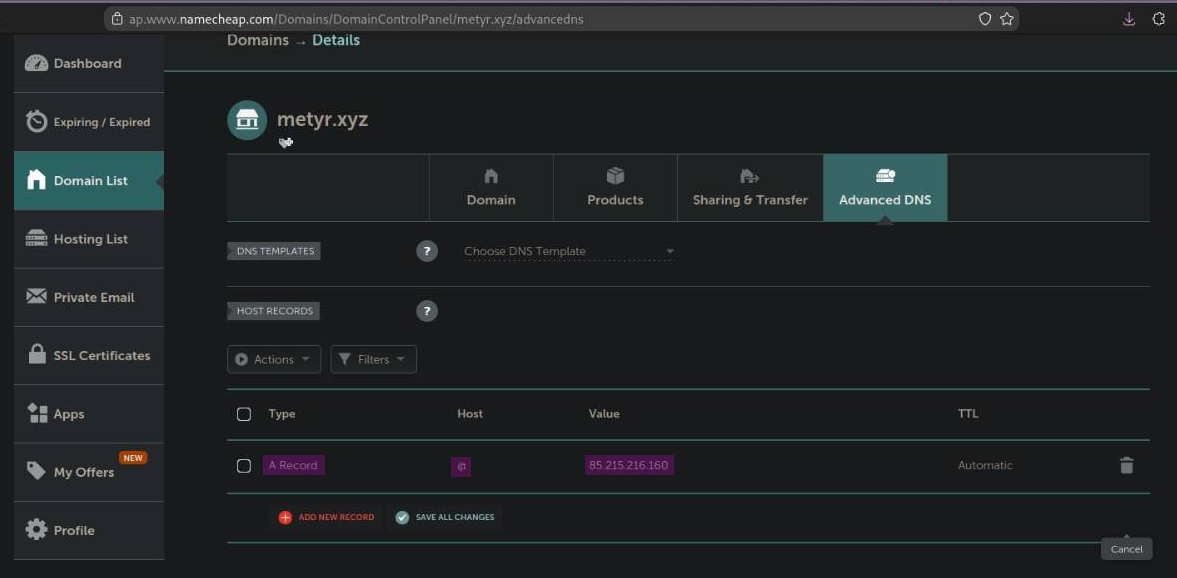
\includegraphics[scale=0.3]{images/dnsentry.png}
	\centering
	\caption{Setting up the DNS record}
\end{figure}\abc\newpage
Lastly, I want to switch from using a self-signed certificate to using an officially signed one by Let's Encrypt. For this, the \texttt{certbot} and \texttt{python3-certbot-nginx} packages need to be added to our system.
Now we can run this command to generate an SSL certificate, which will be signed by Let's Encrypt, so the browser won't give us a security warning anymore.\abc
\texttt{certbot --nginx -d metyr.xyz --non-interactive --agree-tos -m wedm1ebmf@mozmail.com}\abc
The options used are the following:\cite{certbot-options}
\begin{lstlisting}[language=bash]
--nginx #use the nginx plugin for authentication & installation
-d #comma-separated list of domains to obtain a certificate for
--non-interactive #run non-interactively
--agree-tos #agree to the acme server's subscriber agreement
-m #email address for important account notifications
\end{lstlisting}
After running this command for the first time and replying if you haven't saved the certificate, you can use the \texttt{--force-renewal} flag to forcefully renew the certificate in case you lost it or don't want to set up importing it on a rebuild.\cite{cerbot-force-newnew} \abc
If we visit the website now, we can see that we won't be prompted with a security warning. If we inspect the certificate, it will show that it was issued by Let's Encrypt and is trusted.
\begin{figure}[!htbp]
	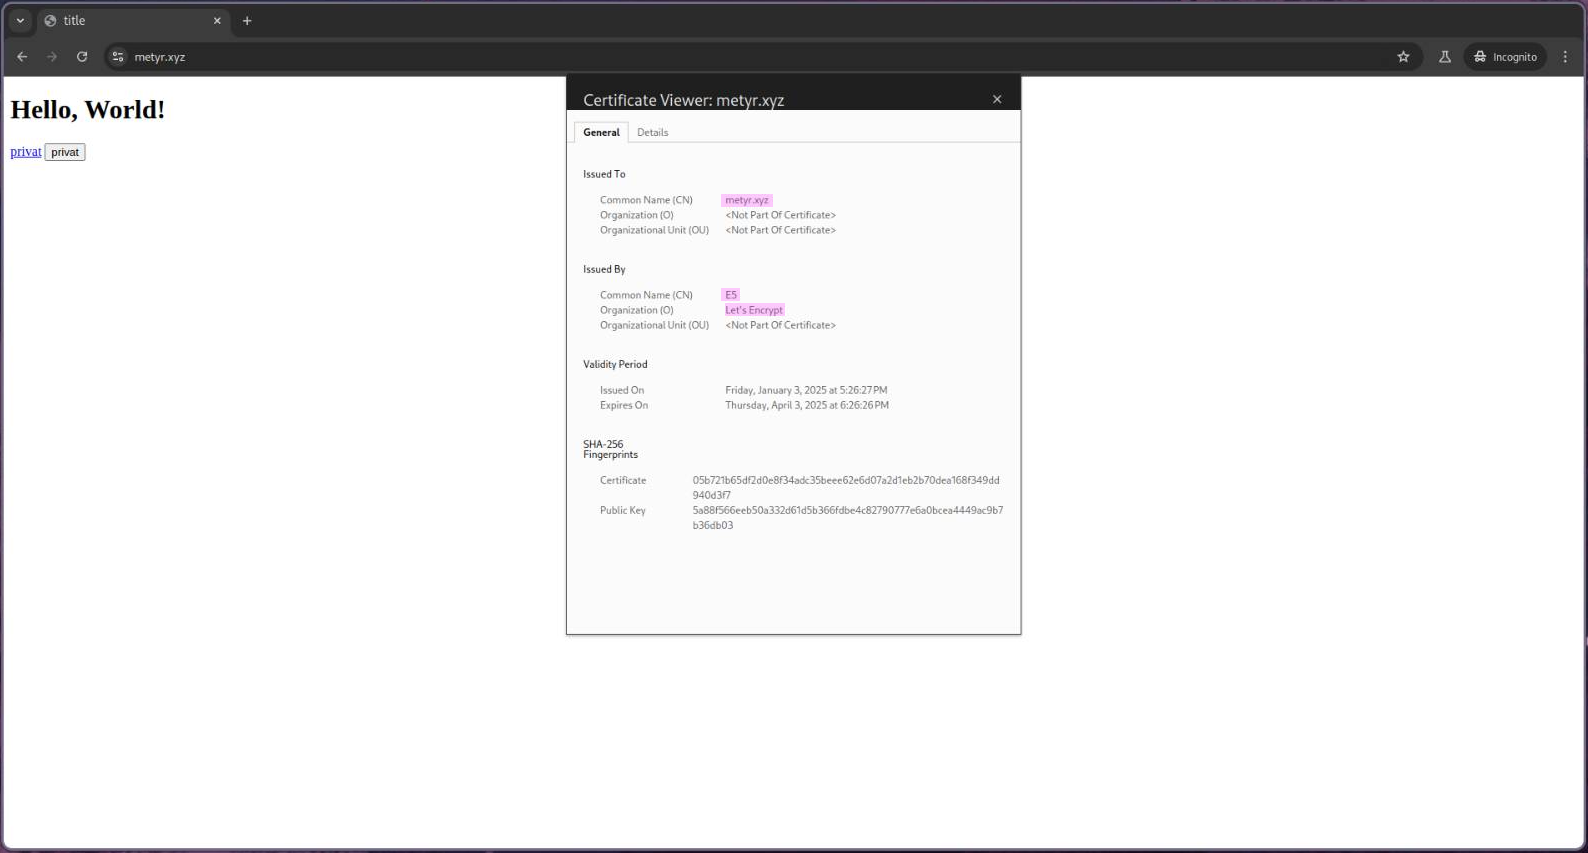
\includegraphics[scale=0.2]{images/nobs.png}
	\centering
	\caption{Showing the trusted certificate signed by Let's Encrypt}
\end{figure}\abc
\newpage
\section{References}
\bibliography{IEEEabrv,quellen}
\newpage
\section{List of figures}

\listoffigures

\end{document}
